% !TEX root = main.tex
\documentclass[main.tex]{subfiles}
\begin{document}

\section{Reducible Power Diagrams}
\label{sec:appendix-nullspace-reducible}

\begin{figure}[t]
  \centering
  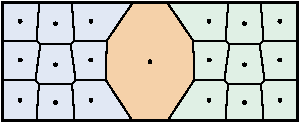
\includegraphics[width=0.49\columnwidth]{figures/nullspace/reducible-cut.pdf}\hfill
  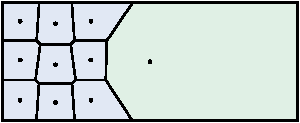
\includegraphics[width=0.49\columnwidth]{figures/nullspace/reducible-cut-coarse.pdf}\\[0.02\columnwidth]
  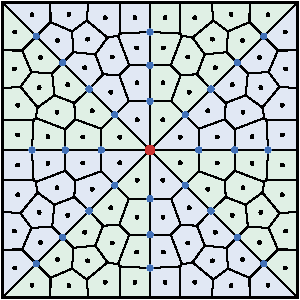
\includegraphics[width=0.49\columnwidth]{figures/nullspace/reducible-dense.pdf}\hfill
  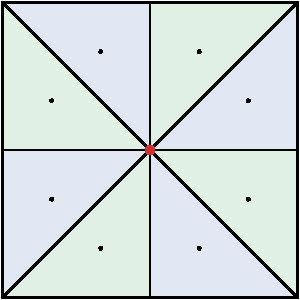
\includegraphics[width=0.49\columnwidth]{figures/nullspace/reducible-coarse.pdf}
  \caption{%
    Two reducible power diagrams (left) and their coarser power diagrams (right), whose cells are unions of theirs.
    Top: generators in general position, whose cut cell (orange) is shared by two blocks of the dual graph, one with the cells on its left (blue) and one with those on its right (green), so that the green cells merge with the cut cell into a single coarse cell.
    Bottom: a Voronoi diagram whose generators are symmetric under the reflections of the square, so that its diagonals and medians are unions of facets, whose vertices are shared by four cells (blue dots) or eight cells (red dot).
    The dual polygons around these vertices make the dual edges within each sector (alternating tints) a class of its own, so the diagram reduces to its eight sectors.
  }
  \label{fig:appendix-reducible}
\end{figure}

We relate here the additional null-space modes of Appendix~\ref{sec:appendix-nullspace-localized} to the concept of reducible power diagrams described by \citet[\S3.4]{Bourne2026ConvexOrder}.
We denote a power diagram with $n$ cells \emph{reducible} if its cells $\cell$ can be grouped into the cells $\widetilde{\cell}$ of a coarser power diagram with $m$ cells, $1 \!<\! m \!<\! n$.
Throughout this appendix, we assume the domain $\domain$ is convex, so that a function that is affine within each cell and convex across every facet is convex on the whole of $\domain$.
% 
Given a coarser diagram with affine functions $\tilde a_I(\xx)$, the perturbation $\delta a_k(\xx) = \tilde a_I(\xx) - a_k(\xx)$, for every $\cell_k \!\subseteq\! \widetilde{\cell}_I$, verifies \eqref{eq:appendix-null-condition}.
However, this perturbation is not a global homothety, since it moves the cells of each coarse cell towards its own affine function $\tilde a_I(\xx)$, while the coarse cells have different affine functions.
Therefore, it corresponds to a localized homothety.
% 
Conversely, let $\delta a$ be a null-space mode with non-constant stretch factors $\kappa_{ij}$.
By \eqref{eq:appendix-kappa}, moving the affine functions along this mode, as $a_k(\xx) + t\,\delta a_k(\xx)$, scales the difference across each facet $\face_{ij}$ by $1 + t\,\kappa_{ij}$, so the cells remain the same as long as all these factors are positive.
As $|t|$ grows, some factors vanish before the others, since $\kappa$ is not constant, which flattens their facets and merges the cells on both sides.
This results in a coarser diagram with $1 \!<\! m \!<\! n$, since some facets have disappeared but not all of them.
% 
Therefore, the null-space modes of $\jointdual$ are larger than the $d+2$ homotheties if and only if the power diagram is reducible, and the classes of its dual graph are its units of reduction.
In general position, a power diagram is thus reducible exactly when it has a cut cell, while dual polygons make it reducible only when they leave additional modes in the count of Appendix~\ref{sec:appendix-nullspace-localized}.
% Moreover, the maximizers of $\jointdual$ with the cells of a reducible diagram form a convex set that extends beyond the homotheties, and that is bounded by configurations in which some generators coincide.
% 
Figure~\ref{fig:appendix-reducible} illustrates both cases.
At the top, the generators are in general position and the diagram is reducible through its cut cell, since contracting the dual edges on one side of the cut cell merges it with the cells on that side.
At the bottom, the power diagram reduces to its eight sectors, and each cycle of four dual edges across a median becomes a single facet between two sectors.

\end{document}
